% \documentclass{IEEEtran}
\documentclass[a4paper]{jpconf}
%\IEEEoverridecommandlockouts
% The preceding line is only needed to identify funding in the first footnote. If that is unneeded, please comment it out.
\usepackage{cite}
\usepackage{amsmath,amssymb,amsfonts}
\usepackage{algorithmic}
\usepackage{graphicx}
\usepackage{textcomp}
\usepackage{xcolor}
% \usepackage{hyperref}
\usepackage{doi}

\usepackage{iftex,ifxetex}
\ifPDFTeX
% \usefonttheme{serif}
\relax
\else
  \ifluatex
    \usepackage{unicode-math}
    \defaultfontfeatures{Ligatures=TeX,Numbers=Lining}
    % \defaultfontfeatures{Ligatures=TeX}
    \setmainfont{Times New Roman}
    \setmathfont{Latin Modern Math}
    \setsansfont{Verdana}
    % \setmonofont{Courier New}[Scale=MatchLowercase]

    % \usefonttheme{professionalfonts}
    % \setmathfont[
    %     Ligatures=TeX,
    %     Scale=MatchLowercase,
    %     math-style=upright,
    %     vargreek-shape=unicode
    %     ]{euler.otf}
  \fi
\fi


% \newcommand*{\doi}[1]{\href{https://doi.org/\detokenize{#1}}{doi: \detokenize{#1}}}
\hypersetup{
    bookmarks=true,         % show bookmarks bar?
    unicode=true,           % non-Latin characters in Acrobat’s bookmarks
    pdftoolbar=false,        % show Acrobat’s toolbar?
    pdfmenubar=false,        % show Acrobat’s menu?
    pdffitwindow=false,     % window fit to page when opened
    pdfstartview={FitH},    % fits the width of the page to the window
    pdftitle={Model Driven Architecture Implementation using Linked Data},    % title
    pdfauthor={Evgeny Cherkashin},     % author
    pdfsubject={model driven architecture},   % subject of the document
    pdfnewwindow=true,      % links in new PDF window
    colorlinks=true,       % false: boxed links; true: colored links
    linkcolor=black,          % color of internal links (change box color with linkbordercolor)
    citecolor=black,        % color of links to bibliography
    filecolor=black,      % color of file links
    urlcolor=black           % color of external links
}

\renewcommand{\doitext}{DOI:}


\def\BibTeX{{\rm B\kern-.05em{\sc i\kern-.025em b}\kern-.08em
    T\kern-.1667em\lower.7ex\hbox{E}\kern-.125emX}}

\graphicspath{{pics/}}

\begin{document}

\title{Construction Techniques of Baikal Microbiome Research Information-Computational Environment}

\author{Evgeny Cherkashin, Alexey Shigarov}

\address{Matrosov Institute for System Dynamics and Control Theory, Siberian Branch of Russian Academy of Sciences, Irkutsk, Russia}

\ead{eugeneai@icc.ru}


% \IEEEauthorblockA{\textit{Matrosov Institute for System Dynamics}\\ \textit{and Control theory of Siberian Branch}\\  \textit{of Russian Academy of Sciences}\\
% Irkutsk, Russia \\
% eugeneai@icc.ru}
% \and
% \IEEEauthorblockN{Alexey Shigarov}
% \IEEEauthorblockA{\textit{Irkutsk Scientific Center of Siberian Branch} \\
% \textit{of Russian Academy of Sciences}\\
% Irkutsk, Russia \\
% shigarov@icc.ru}
% \and
% \IEEEauthorblockN{Vasily Khristyuk}
% \IEEEauthorblockA{\textit{Natinal Research Irkutsk} \\
% \textit{State Technical University}\\
% Irkutsk, Russia \\
% khr@icc.ru}
% }

%\maketitle

\begin{abstract}%\color{red}
A tool set and model data sources for research and developing an environment for Next Generation Sequencing data processing are considered in the paper.  The environment is constructed on the base of model transformations targeted to industrial grade systems allowing domain specialists to carry on the NGS research, which includes genetic data processing, visualization, and data integration.  The integration allows one to get rid of restrictions imposed by an application library by its operation set and properties.  The technique of the transformation is based on Model Driven Architecture principles and logical inference of the derived models and the code.  The current results and the future fork are presented and discussed.
\end{abstract}

% \begin{IEEEkeywords}
% next generation sequencing, big data, model driven architecture, linked open data, problem solving
% \end{IEEEkeywords}

\section{Introduction}
%This document is a model and instructions for \LaTeX. Please observe the conference page limits.

%Baikal microbiome research is a relatively new activity of Limnological Institute of Siberian Branch of Russian Academy of Sciences (LIN SB RAS).  In the Cell ultrastructure laboratory the microbial investigations are based on ... as well as Next Generation Sequencing (NGS) approaches based on analysis of amplicons.

In the last decade after the invention of methods for sequencing of new generation and their introduction in practice of biological systems research, a new direction of molecular genetics is formed, which is referred to as \emph{metagenomics}. Its main object of study goes beyond the individual microscopic cultivated organisms to their communities, \emph{microbiomes}. A total DNA is extracted from a sample, resulting in a general image of the microbiome. The method allows one to describe a significant number of new groups of organisms at all taxonomic levels. A comprehensive review of present sequencing approaches and challenges are described in \cite{pere20}.

One of the types of the metagenomic studies is the \emph{analysis of amplicons}. Analysis of amplicons is applied to investigation of the microbiota of different environments of Lake Baikal \cite{underice}. To perform the analysis, significant computational resources are required, as well as bioinformatics skills for analysis and interpretation. The Researcher composes the computational process by combining different modules of bioinformatic software, data conversion, data analysis, and visualization. To carry on the studies, the domain specialist are required to be skilled in scripting of the command shell of the operating system (Linux, Windows), running a distributed computing environment, a cluster computing systems, and programming general and domain-specific languages, \emph{e.g.}, Python and R.

The aim of this study is to develop mathematical and software support of the processes of analysis of the results of Next Generation Sequencing (NGS). We are to develop and implement techniques and software for visual representation of the computational process of amplicon analysis so that domain specialists would be able to compose computational pipelines, which are executed in distributed heterogeneous computing resources (clouds). Software implementation is a cloud infrastructure built on models of representation of the computational process in the form of a set of operations, structure and functions of the computing resources, and scheduling algorithms for computational resources.

In \cite{guo16} the problem of cloud usage for storage and computing is stated as the basic problem of NGS, since storage capacity exponential growth is slower as compared to the growth of the NGS generated data volume. The transportation between the mirror storages and the computer systems for processing data could easily cause the network capacity exhausting. The data processing in the general case of whole genome reconstruction requires terabytes of RAM and, in the case of cluster computing usage, special high performance parallel algorithms. Two classes of users identified: \emph{power user}, who analyses the genome, and \emph{causal user}, who deals with the power user results, \emph{e.g.}, integrating gene data between datasets and studies.


% Our case

The domain of our IT R\&D is related to processing data within natural science research activities, which are characterized with varieties of tasks, methods and the multidisciplinary aims. % TODO: Double it in Related works.
We are observing constant increasing of the data obtained from field investigations, each new data is compared to all the data obtained in the previous years. The number of scientific problems is being increased too. Another problem to be solved is the interest of domain specialists, biologists, to be involved in data processing, guaranteeing a reasonable quality of processing.  This processing pipeline should be automatic in general and be adjustable in therms of math- and biodomains.

We propose to construct a PaaS and DaaS cloud consisting of independent network connected SaaS-services adopted for MiSeq standard operational procedure (MiSeq SOP) used in microbiome research of Lake Baikal. PaaS will enable biologists to investigate data themselves, DaaS will allow bioinformatic specialists to work with data on demand when designing new data processing techniques, and SaaS services will support the individual operations for PaaS. There are a number of SaaS software already made for NGS data processing, ref.~\cite{guo16} contains their detailed survey. % realized mostly with Mothur software package\cite{mothur

% Visualization ...

\section{Automation of MiSeq standard operational procedure}
\label{sec:sop}

To be more concrete in the further reasoning, we briefly describe MiSeq SOP implemented with Mothur software \cite{mothur}.  NGS data analysis process consists of the individual operations on genetic data, which are stored in files. To get accounted with the technique, we tried to process limnological data \cite{mik19} according to procedure presented on \href{https://www.mothur.org/wiki/MiSeq_SOP}{Mothur website}\footnote{\url{https://www.mothur.org/wiki/MiSeq_SOP}}. %%% Input data, gene data readings, are taken from GS FLX454 sequencer were given as initial data.

% We started from summarizing initial \verb|fasta|-file filled with 44934 \emph{contigs} (contiguous gene sequences). The Next operation is trimming \emph{oligos primers}, a sequence parts identifying samples for each contig. After each trimming, filtering and alignment operation, the researcher is to observe summary statistics on the \verb|fasta|-data of readings. The summary data are represented as statistic criteria of minimal, maximal, average and four-quantile evaluations. This allows researcher information to figure out parameters for next operations.

% After trimming oligos, one must remove shorter- and longer--than--average sequences. The degree of deviation is usually determined by the percentage of readings allowed to be removed. In our case, we removed 11052 (25\%) shorter readings. The Next step is figuring out unique sequences and count their replicas. This allows us to carry on the following steps once per unique sequence, resulting in reduction of computational time. We obtained 26744 unique sequences, which have been passed through screening filter, removing sequences with \emph{homopolymer} characteristic being more than 8. The longer sequences of the same base pairs in a row, homopolymer, will not exist in nature.

% Main computationally complex stage of a sequence analysis is their \emph{alignment} with data stored in a reference gene database, \emph{e.g.}, SILVA \cite{silva}. Applying the alignment to our 21170 sequences changed lengths of readings from average 407 to exact 871, filling them with gaps. After trimming ``hanging'' readings characters and filtering unaligned ones, we applied again selection of the unique sequences, resulted in 21052 unique ones. As optional step, we ``relaxed'' the difference between sequences allowing one additional mutation per 100 base pairs, reducing their number to 14234.

% Next step is \emph{chimeras} detection and removal. Chimeric sequences are contigs constructed from rRNA partial readings (right-to-left, left-to-right) of different species, but having common parts. This stage is based on construction of a classifications and assignment of the readings to the classes.  The very rare instances of readings are considered to be chimeric and removed. This stage is mandatory, and the amount of rejected sequences must be evaluated. We obtained 11119 unique sequences, 1.3\% of total number (a reasonable amount), thus, the initial data were reduced to its 25\% number of readings.

% After this stage we can make one final filtering, removing mitochondrial and chloroplast rRNA. To do so, the unique sequences must be classified. The classification is carried on with a trained Baesian network. In our case, we removed 1828 sequences, and the final set of sequences contains 9291 unique readings.


% \subsection{Microbial community analysis}
% \label{sec:biome-anl}

% There are four main analyses carried over the processed sequence sets (groups, samples). The sequences are organized in \emph{operational taxonomic units} (OTU), which could be thought as an abstraction of a ``genus'' notion, they could have determined taxon or not. OTU contains sequences, which have a predefined mutation level usually not over 3\%. For our data we obtained about one thousand OTUs.

% The first microbial community analysis is a determination of the abundance of the recognized bacteria by their taxons levels in each OTU. The second one is phylogenetic analysis aimed at detecting the mutation distances between the OTUs. The third one, named Alpha-diversity, deals with representation of the similarities of the groups (samples) on the base of inhabiting OTU and sequences and vice versa (similarities of the OTU on the base of groups). Heatmap charts are built (Fig. \ref{fig:heatmap-ex}).

% \begin{figure}[bt]
%   %\centering
%   % 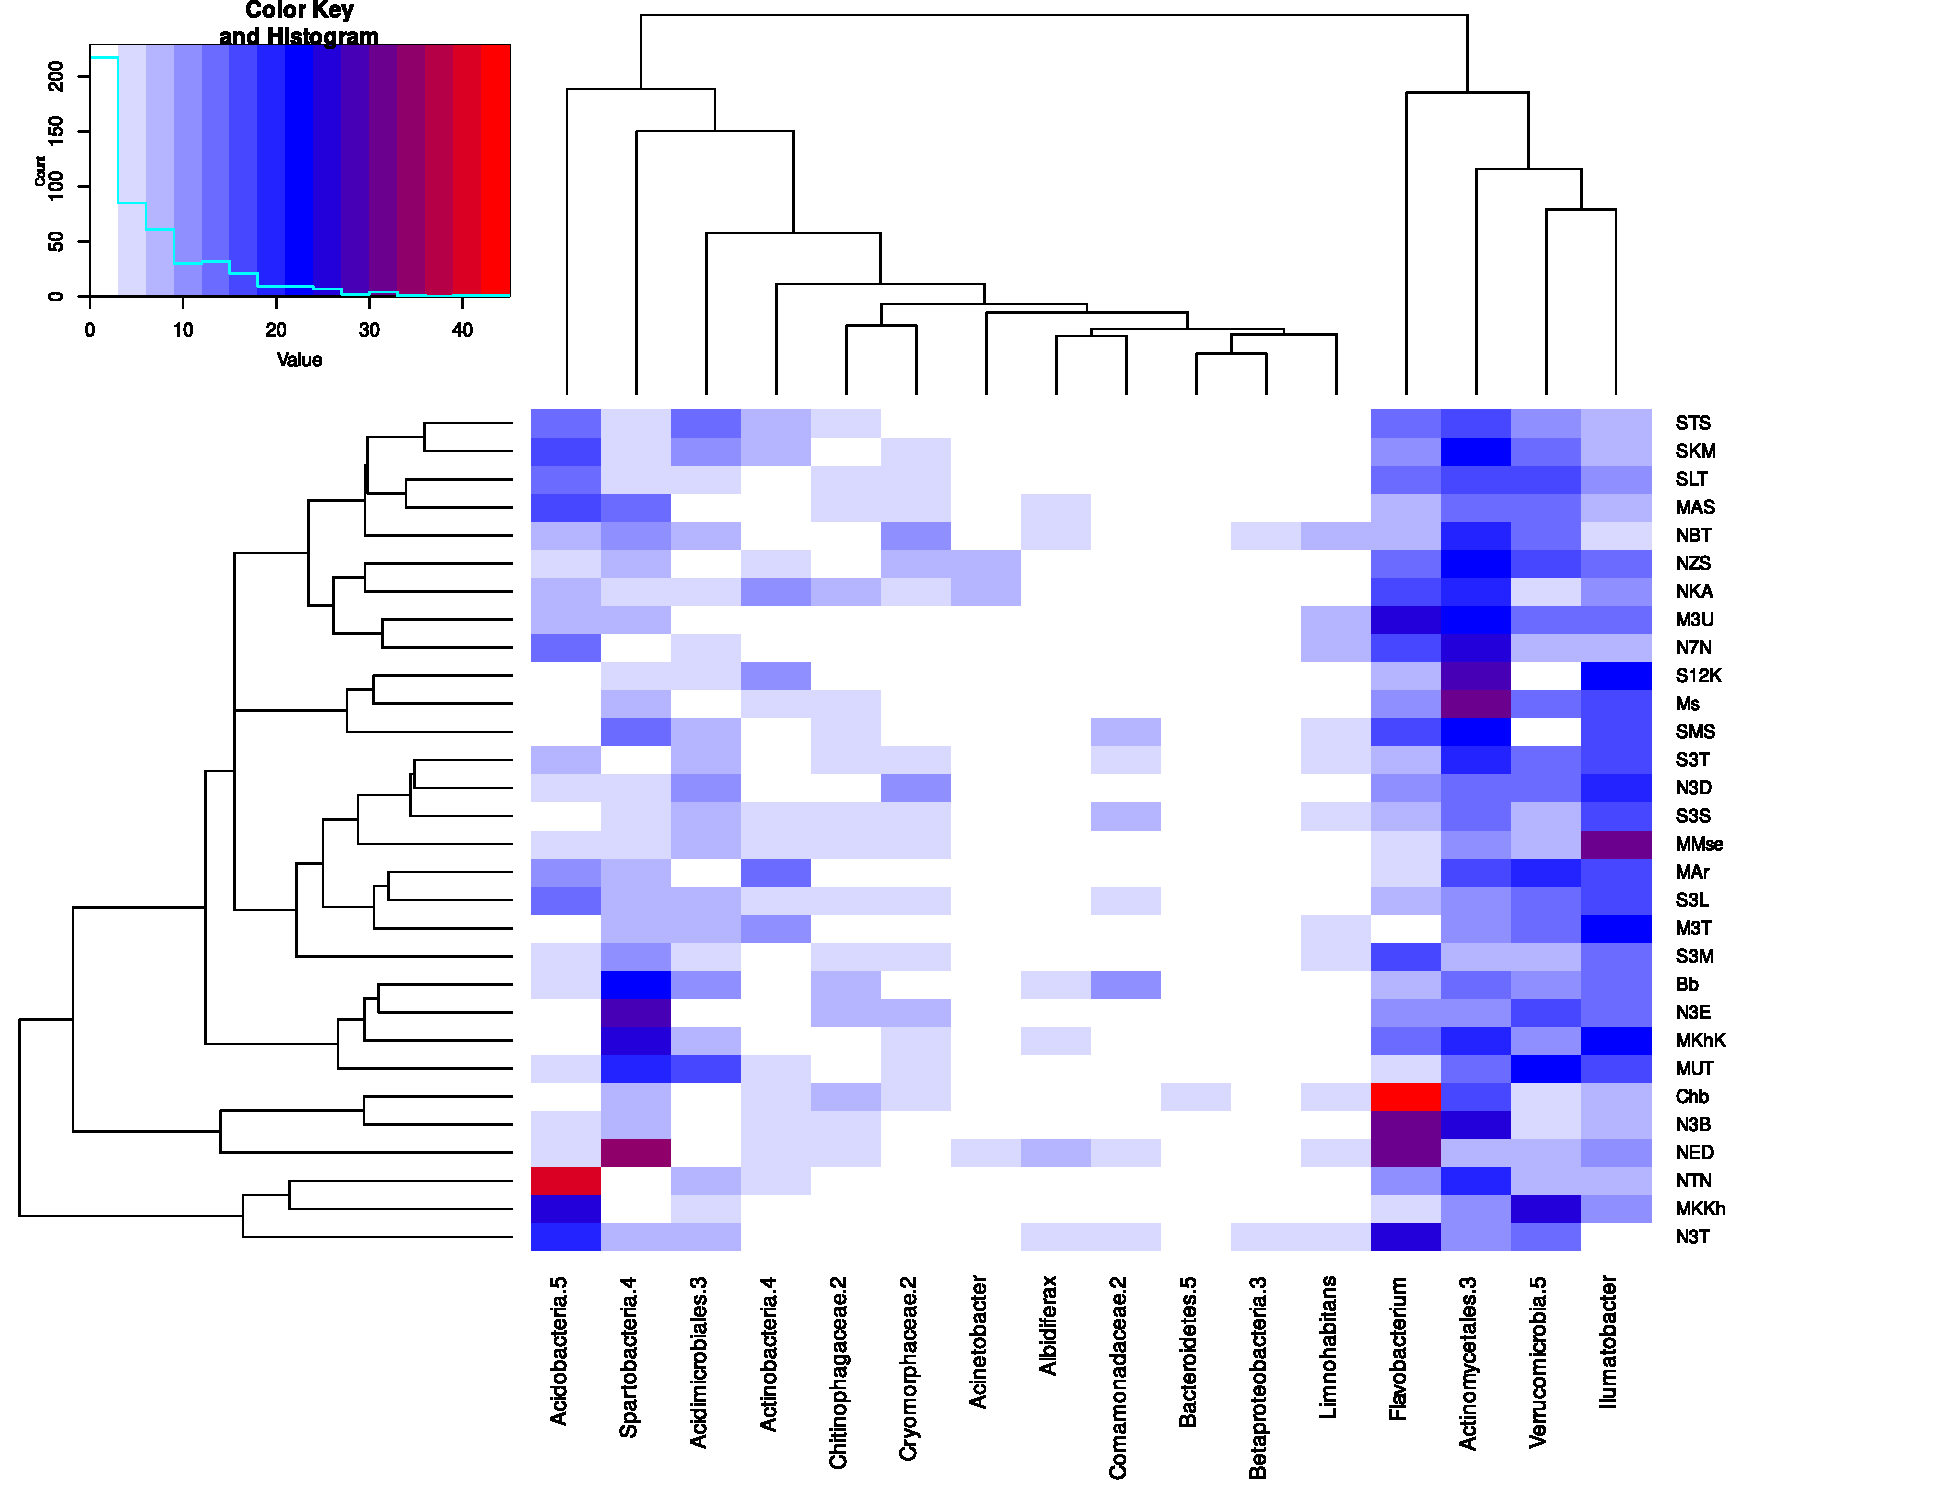
\includegraphics[width=1.1\linewidth]{heatmap-OTU-Group-tax.pdf}
%   \caption{An example of a heatmap diagram}
%   \label{fig:heatmap-ex}
% \end{figure}

% The fourth analysis is referred to as Beta-diversity, which deals with principal component analysis and its analogs, constructs charts of group by similarity in the space of the principal component axes. The number of representing axes are determined sequentially adding one by one and analyzing change of the $R$-criterion and the stress.

%%% \subsection{Technique manual implementation issues}
%%% \label{sec:finnotes}

After executing the technique manually, we observed a number of issues. Parameter structure and output of a Mothur command is intricate: researcher needs to trace file names change from a command to the following one.  After each execution, a Mothur command adds suffixes to the input file names.  File naming depends on the input parameters, \emph{e.g.}, method used to process data. For example, after application \verb|align.seq| to file named \verb|HXH779K01.shhh.trim.good.unique.fasta| we obtain\footnote{File names are truncated in the beginning for better text layout.} \verb|HXH779K01.shhh.trim.good.unique.align|, \verb|HXH779K01...trim.good.unique.align.report|, and \verb|HXH779K01...im.good.unique.flip.accnos|.  Almost each operation adds new suffixes.  Repeating application of an operation to data results in repetitive suffixes.  Mothur can pass correct filenames itself if the process goes directly forward, \emph{e.g.}, in scripts.  Making a mistake or returning to a previous step to refine coefficients, researcher must trace the filenames manually.

After obtaining the results in the forms of tables and charts biologists usually repeat some filtering stages excluding additional OTUs, \emph{e.g.}, which is similar to mitochondrial and chloroplast, but were not recognized within MiSeq technique.
%%%
Sometimes users want to replace a command with analogous one from another package, \emph{e.g.}, QUIIME2 or Usearch, to check the default one or take advantage of special features of the external command. In this case data conversion must be performed.
%%%

Another possible but less frequent deviation from the technique is the involvement of the previously processed OTUs from early research, \emph{e.g.}, samples of the previous year in the same places during ecological monitoring. In this case, researcher needs to match the OTUs from different studies. User should write a routine for comparing OTU contents and merging group data.
%%%

Visualization is partially presented in command set of Mothur.  It is able to produce SVG vector images, but the images in general cannot be customized.  Researchers have to use external software like R to build charts of the desired quality.  Our experience show that despite the time spent to study the chart building techniques, which is needed once, most time spent for converting and filtering input data and refining parameters of the chart building commands.

\section{Related works}
\label{sec:relworks}

Main R\&D activity in the NGS domain are divided on three main directions: development new efficient algorithms for data processing operations and building charts, organizing standardized cloud computing pipelines with HPC implementations of various operations, and representing pipelines as workflows, as well as user interfaces to support interactive data processing and assessment.

At first, let us consider research devoted to the productivity of the algorithms and improving the analysis results quality.  In \cite{const19} Go, C++ and Java programming languages were assessed with respect to the ease of implementation, memory consumption and overall computation performance, Go was chosen. Main requirements were addressed to big data string processing. The system designed to store string under processing in main memory, share data parts between CPUs and limit input/output operations. Interesting is the fact that C++ was the slowest.

In \cite{Gong16} a NGS analysis pipeline was developed for analysis viruses' DNA contained in human body. This analysis allowed medical engineers to focus studying on vaccine development. These findings demonstrated that the proposed NGS data analysis pipeline identified unknown viruses from the mixed clinical samples, revealed their genetic identity and variants, and characterized their genetic features in terms of viral evolution. The process of detection is based on comparing parts of viral genome with BLAST database and the coverage analysis.

Paper \cite{grass12} deals with implementation of a heuristic algorithm for \emph{scaffolding}, \emph{i.e.}, ordering, moving and orienting contigs using additional information to produce longer sequences on the next stages.
In \cite{muller16} a data-driven user interface and visualization is considered in the process of a clinical decision support system implementation. The user interface supplies decision-making for doctor and explanations for patients as list of events of various kinds (medical records, NGS results over autopsy tissue, \emph{etc.}) represented as HTML5 portlets. A comprehensive review of quality control, error correction and detection while processing NGS data is presented in \cite{te16}. %, it would be of purpose to implement them [within our software].

The HPC techniques review we will start with application of BOINC technology to alignment presented \cite{boinc10}, where Novoalign algorithm was scaled.
The reference \cite{guo16} reviewed the problem area, described the existing approaches and services already made, but has no mentions of the implemented cloud computing environments.
%
Paper \cite{kwon15} contains an excellent review of current achievements in NGS and related areas. Authors doubt about the possibility to organize a laboratory HPC-center based on cluster computing by NGS software users and suggest dealing with IaaS cloud computing. The paper has very good review of existing commercial and open-source platforms allowing construction of pipelines of computing processes. Commercial software mostly implement predefined pipelines and inflexible, whereas open-source tends to implement either standardized pipelines or present a set of modules for individual operations and cloud service implementations, a \emph{toolsets}.
%
In \cite{zhao17}, Raibow software, a cloud implementation of NGS data processing, is considered. Rainbow is essentially a Perl script implementing map (division) for input and reduce (join) for output data, together with distribution of the data pieces between Amazon EC2 cloud nodes. Cloud nodes perform only alignment. The paper also has a good review of Linux virtual machine cloud distributions and bioinformatic packages.
% % Common Workflow Language... CWL
Another interesting review of cloud computing techniques is presented in \cite{lang18}. Authors pay attention to open-source cloud (Open Stack) and construction tools, like Common Workflow Language (CWL) \cite{cwl} used to represent the computational process in a cloud.
A comprehensive short survey can be found in \cite{baker18}, but at this point, it will not add essential data.

There are visual tools for genetic analysis, \emph{e.g.}, Galaxy \cite{galaxy18}, which implements popular approach (metaphor) of interactive web page, where data are imported and processed with modules. Galaxy also can analyze the user script and constructs \emph{dataflow} representation. Its primary purpose is to teach biologists to process single genome data, it can be extended to implement other NGS research. This is open-source project, under active development, and we could use it as one of implementation platform. Another tool is UGENE \cite{ugene18}, it is a desktop application, open-source, written with QT5 framework, and also under active development. UGENE primary visualizes workflow and gene data. Main criticism of the tools is presented in \cite{mill16}, where it is stated, that command line utilities support more functions and have higher flexibility than visual tools. Authors propose own visual tool VisPro, connected to a cloud. The tool is build on the base of agile approach, which assumes principal participation of developer the process of workflow construction, configuration and execution.

Summing up review, we conclude, that there are good background to construction of our infrastructure, and the techniques used in Baikal microbiome research must be adapted to this background. The technologies we spoke before allow us to account the peculiarity of our problem, which is the requirement of a greater flexibility of the computation process and domain user experience adaptation.
%%% Summing up this short review, we conclude, that there are good background to construction of our infrastructure, and the techniques used in Baikal microbiome research must be adapted to this background. The technologies we spoke before allow us to account the peculiarity of our problem, which is the requirement of a greater flexibility of the computation process and domain user experience adaptation.



% \section{NGS data processing software}
% \label{sec:ngs-soft}

% Let us consider structure of the NGS data processing on the example of Mothur software, which probably contains routines for all popular operations of NGS data processing, as well as support loading and generation files of the popular formats.

% ...

% Mothur's data processing algorithms account the existence of multicore CPUs.

\section{A MiSeq SOP automation approach}
\label{sec:proc-mod}

Limnologists perform both power and casual users activities \cite{guo16}, \emph{i.e.}, processing both raw sequencing data and the result of the sequence processing, visualizing, comparing and generalizing results. High performance computing is usually based on two popular programming models \cite{guo16}: MapReduce (Hadoop) and task programming. The first one implies that data can be split in subsets, which could be processed mostly independently. The results of the parallel processing, then, joined (reduced) to an aggregative object.

 Mothur's simple filtering commands are easily run in parallel, indeed it uses CPU cores, but the computational complexity seems to be not as high as it would be reasonable to spend time on splitting and joining.  Main reason using clouds here is the accumulation of the RAM if data would not fit in the workstation memory. % In this case Mothur processes data by sequential reading fasta sequences (strings).
Some filtering is based on classification, which processes the whole gene data using subsampling.  Transition of the corresponding algorithms to SaaS implies their substitution to a cluster versions.

In general, to make our cloud computing architecture simpler, at the first stage of R\&D we decided to use \emph{task queue} execution model, where computational resources execute individual tasks from a network of modules representing a variant of MiSeq SOP.  The network of modules is constructed on the base of a MiSeq SOP model, where each module is a module of Mothur package.  The network is designed with Rapidminer studio as a dataflow. In Fig. \ref{fig:mothur} we represented the beginning of the MiSeq SOP.  Integration with cloud will require transfer data between DaaS and SaaS, store objects with metadata, and this is also accounted in our model.


%\subsection{Dataflow model of MiSeq SOP}
%\label{sec:miseq-model}

%Let us consider the modeling Mothur as a dataflow.

\begin{figure}[bt]
  \centering
   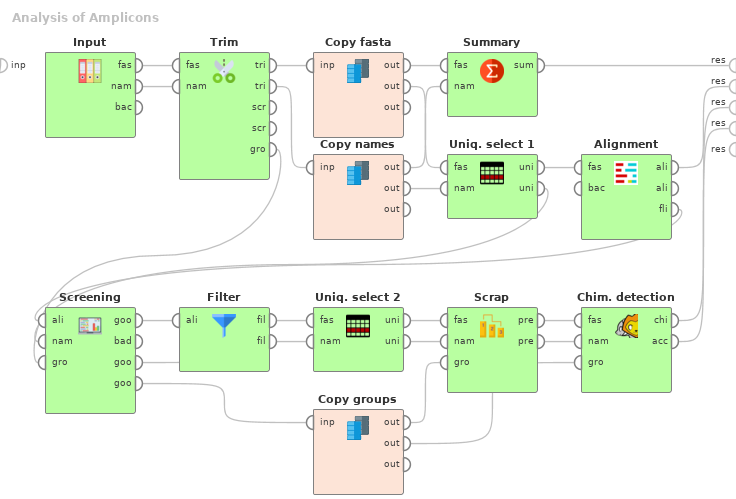
\includegraphics[width=0.7\linewidth]{Dataflow-color-en.png}
  \caption{MiSeq first stages representation as dataflow modules \cite{cherk19}}
  \label{fig:mothur}
\end{figure}


\section{Implementation concepts}

The review of papers shows that as of to date there are two open-source projects related to automation of NGS data analysis being in active development: Galaxy and UGENE.  If take Galaxy as the main data processing visualization technique, we are to make Galaxy modules adapting Mothur command, as well as adapt Galaxy visualization techniques to the MiSeq SOP.  On the other hand, we can do the same for UGENE, allowing user to work with more responsive dynamic interface of the UGENE desktop application.

%%%% Repeats the previous one
%%%Our review reveals a number of opens-source projects to be useful in R\&D of our project.  Galaxy project is of our primary interest as it provides standardized and significantly implemented data processing visualization techniques.  Galaxy module sets (tool sets) contain Mothur operations and their formal description, which could be used to refine our knowledge base of model transformation.

In \cite{cherk19} and \cite{zont19} we proposed and implemented a technique for dataflow representation of all Mothur commands.  We use Model Driven Architecture (MDA) to generate modules for Rapidminer studio, a visual dataflow editor.  According to MDA, the source code of modules are generated from so-called Platform Specific Model (PSM), which represents the software under development in a notation allowing the direct code generation by means of templates and other simple procedures.  In our case PSM represents Java source code of the dataflow modules.
%%%
%The source model, so called Computationally independent model, is obtained  automatically from the analysis of the C++ source code of Mothur.  The resulting source code represents Java modules defining parts of a dataflow diagram.

PSM is built out of Platform Independent Model (PIM) representing the software on a more abstract level than PSM.  It expresses the relations between entities, their object structures, metainformation and so on.  Transition from PIM to PSM (a model transformation) is carried out by means of logical inference of the PSM properties on the base of facts representing PIM and the properties of the implementation platform, a Platform Model (PM), in our case it is Java programming language.

Some properties of PIM, \emph{e.g.}, list of object fields, are constructed by transformation of Computationally Independent Model (CIM), an even more abstract model, which represents software as entities of the domain of Mothur commands.  The transformation is also implemented as logical inference realizing a pattern recognition.  The CIM is also obtained automatically from the analysis of the C++ source code of Mothur. The analysis is implemented as a Python program scanning the sources for a specific structures.  Each command implementation is analyzed with set of regular expressions matches organized in a scenario.

\subsection{RDF data representation}

The source model data are represented on the base of Semantic Web technologies.  The model and its comprising structures are identified globally as resources.  Relations between resources and literal values are expressed using standard and \emph{ad hoc} designed ontologies.  Usage of the ontologies allowed us to direct the research ``along known spaces'' of metadata and use the experience of the designers of ontologies, narrow the search space of the solutions.

%%% ---- a short version ----
%We adapted a number of standardized ontologies. Friend-of-a-friend (foaf) ontology is used for agent information: individuals, legal entities, program agents; Provenance (prov) is used for making references between documents; Dublin Core (dc) is used for published resources' metadata mark up; DBPedia resource ({dbr}) refers external globally used classes and instance objects; Open annotation ({oa}) is used as a published document content representation ontology; \emph{etc}. Used approach allowed us to solve many technical problems, including providing dataflow visualization tool Rapidminer Studio with an actual set of Mothur commands, implementing an abstract engine of Mothur command properties mapping to a software environment.

In the cloud DaaS, we are to store files and its contents as object with its metadata.  The nowadays OMG\footnote{Object Management Group} standards describe specifications of converting relational, UML, SysML metadata to RDF representation.  So, we can store data in conventional relational or key-value databases and while retrieving supply metadata as well.  In the simplest case, data and metadata can be stored in metadata storages, such as ClioPatria.  While designing our cloud storage we use the JHipster Domain Language \cite{jhipster} and its tools to create database structures, metadata converters, formal representations of the ontologies of the stored data.

% LOD

Metadata of the database stored objects describes mostly relations between a resource and its attributes.  Some attributes, namely foreign keys, are the references to other resources, which also reflected with metadata.  There are rare relations between resources, which are not stored in the conventional databases.  These relations reflect, \emph{e.g.}, data provenance, additional special attributes for a particular data object.  Such rare relations are infrequent and can be added in a special research investigation, so modification of the relational database structure for each of the case has no sense. For representation of the data, we adapted a number of standardized ontologies. Friend-of-a-friend (foaf) ontology is used for agent information: individuals, legal entities, program agents; Provenance (prov) is used for making references between documents; Dublin Core (dc) is used for published resource metadata mark up; DBPedia resource ({dbr}) refers external globally used classes and instance objects; Open annotation ({oa}) is used as a published document content representation ontology; The Bibliographic Ontology ({bibo}) is used for literature reference mark up; \emph{etc.} For representation of Mothur CIM and PIM, we developed two ontologies \texttt{mothur} and \texttt{uml} (for XMI model data representation).  CIM and PIM ontologies are used to represent relations between stored objects as subjects of input and output of Mothur commands.

Used approach allowed us to solve many technical problems, including providing our dataflow visualization tools with an actual set of Mothur commands, implementing an abstract engine of Mothur command properties mapping to a software environment. Within the R\&D, we obtained a set of transformation scenarios expressed as object knowledge sets represented in the Logtalk \cite{logtalk} programming language, which can be used to generate PSM and the source codes for representation of Mothur command for new computation and visualization environments.

\subsection{Data integration: Metadata inference}

To allow a casual user to take advantage of the obtained results, they are to be represented as RDF/RDFa marked up report documents (Word, Excel, PDF) and HTML5 web pages, \emph{e.g.}, produced by Galaxy software.  Such format allows both the user and a software agent to acquire the resulting data for their research.  The markup for the documents is a part of our LOD-based service providing integration with other NGS Internet resources.  At present, we have not found a standardized way of the integration: there are only prototypes of annotation resources, like BioSearch \cite{biosearch} implemented on the base of BIO2RDF LOD technologies.

The LOD service and the required flexibility of scientific research software requires us to associate metadata to all pieces of NGS data.  The metadata is stored for main input data of MiSeq SOP and transformed with each application of commands into metadata describing command output objects.  For Mothur, we construct an automatic metadata inference rules analyzing its C++ source and filename conversion algorithms.  To conserve memory usage we decided to implement dynamic metadata reconstruction when DaaS returns queried objects.  For example, as thousands of sequences are organized in files, groups and OTUs, the metadata of the sequences are extended with all file/group/OUT metadata, each sequence metadata is generated using the context of its storage, namely \verb|fasta|--file name and relation to its group, its file provenance, \emph{etc.}


\section{Further development}

To date we developed means for MiSeq SOP modeling with dataflow diagrams in Rapidminer studio, execution of the models as creating scripts in Mothur simple scripting language, together with MDA instrumentation support. The main problem to be solved in the future is as follows:
\begin{itemize}
\item development of a converter of the models into Galaxy scenarios;
\item integrate data storage with Galaxy data import subsystem;
\item implement metadata storage and adapters for NGS data;
\item create a more sophisticated source code parser or PIM model of computation, so we could be able to infer metadata for synthesizing metadata conversion rules;
\item adapt our document authoring tools to Galaxy allowing LOD representation of results;
\item implement integration to biological/gene databases;
  % \item Write a handbook on Logtalk programming strategies with its author Paulo Mora.
\item develop a set of predefined scenarios,
\item create scenarios templates which will support research in monitoring.
\end{itemize}
The target modular software architecture is presented in Fig.~\ref{fig:metadata}.
\begin{figure}[bt]
  \centering
   % 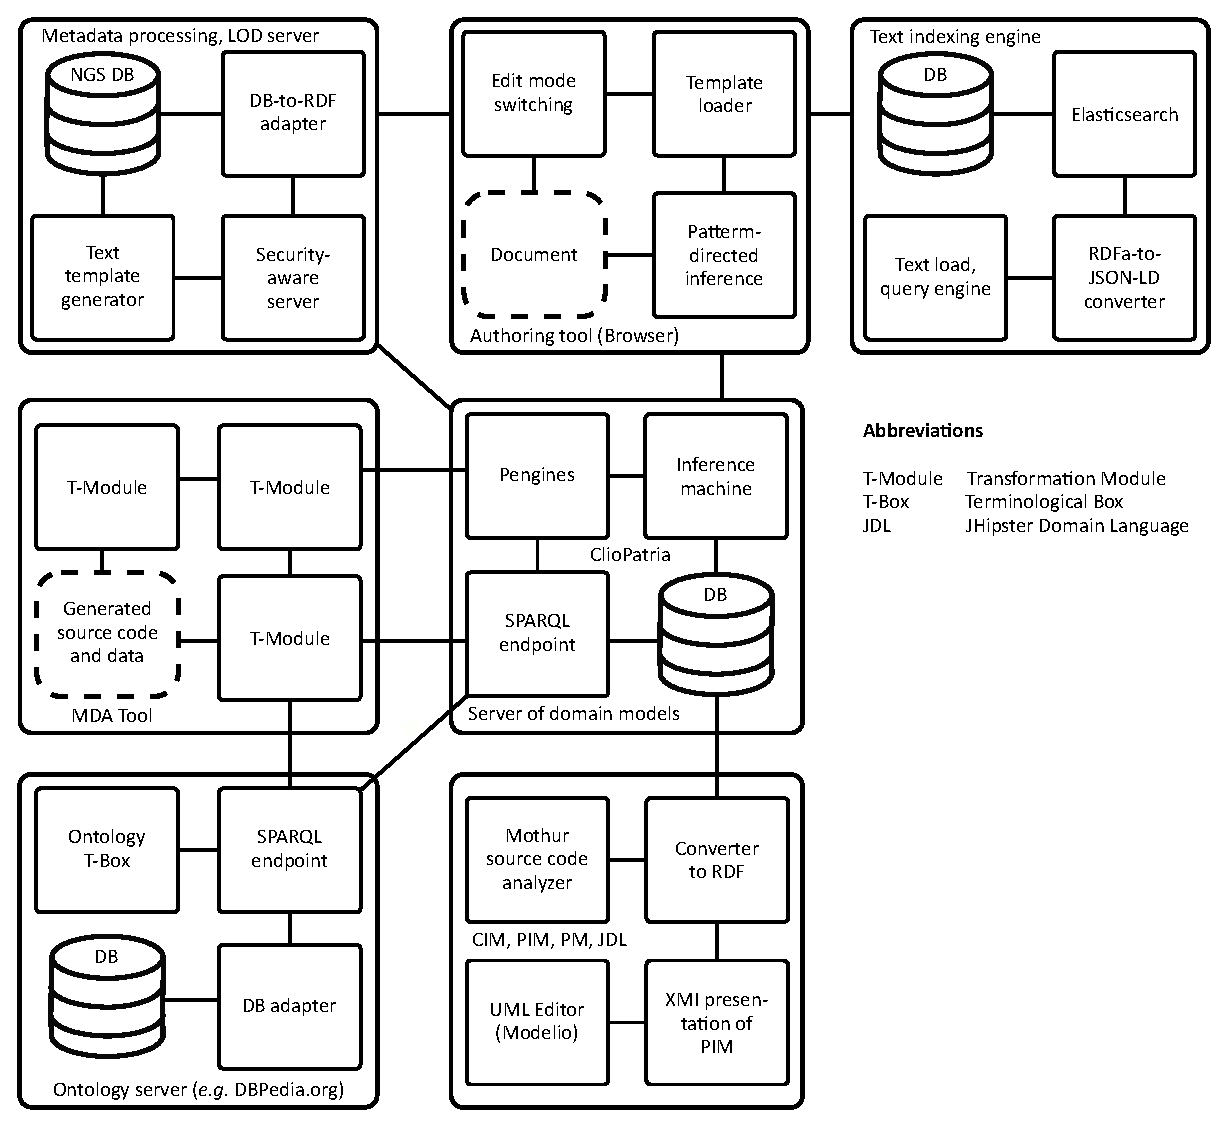
\includegraphics[width=1\linewidth]{architecture-mda-lod-ext-ngs.pdf}
   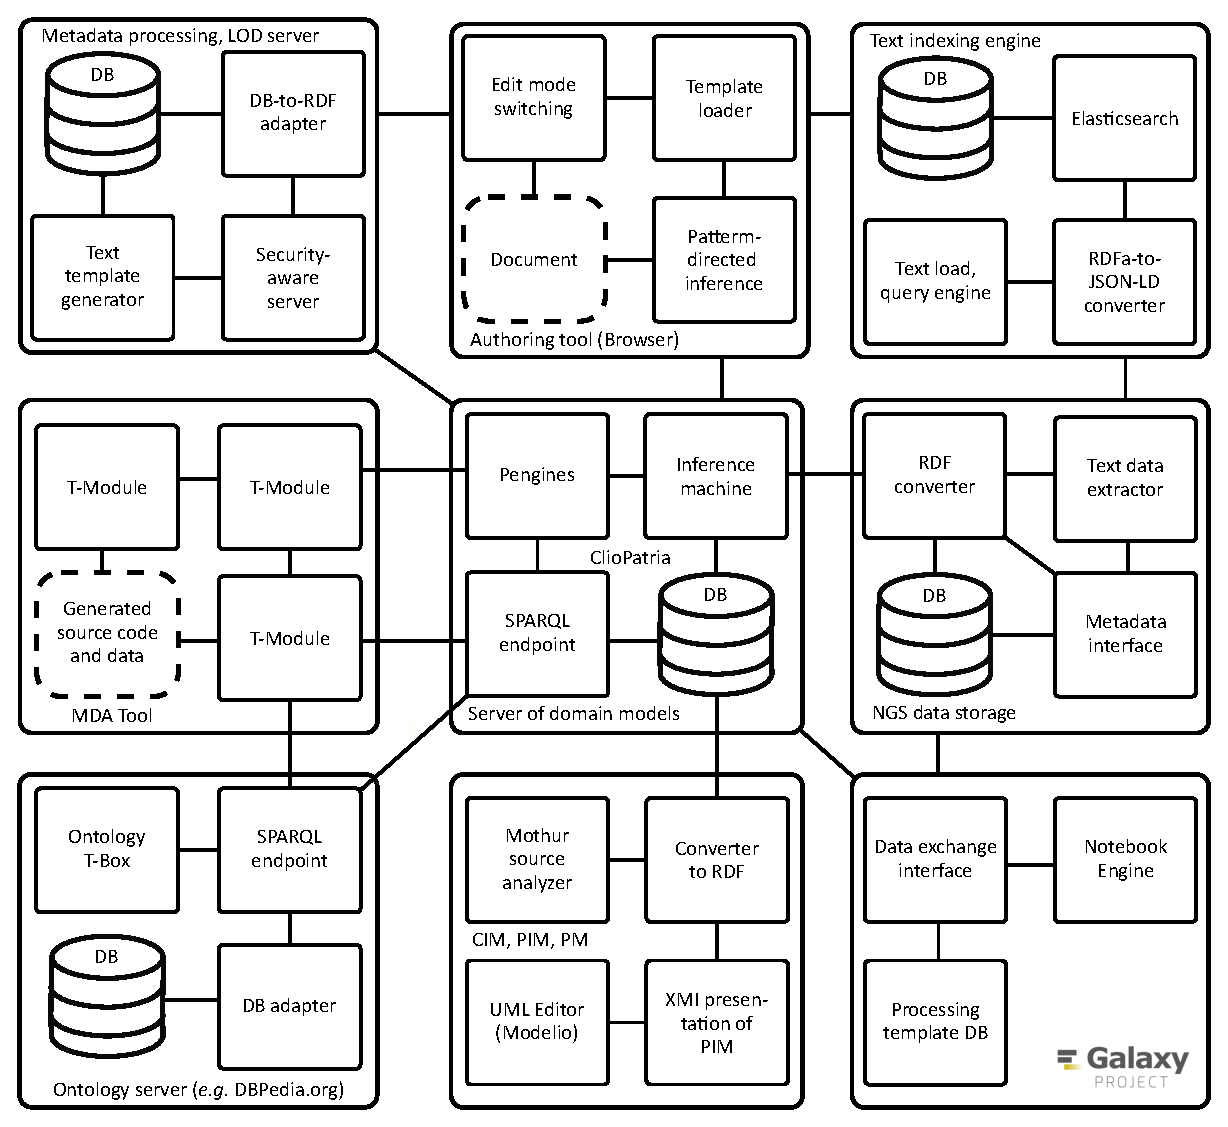
\includegraphics[width=0.8\linewidth]{architecture-mda-lod-ext-galaxy.pdf}
  \caption{Architecture of information-computation environment}
  \label{fig:metadata}
\end{figure}

% \subsection{Model Data representation}

% Idea of RDF representation

% LOD and its document-relation....

% Used ontologies


% \section{Dataflow Mothur command model}
% \label{sec:datflow}

% General idea of integration of Mothur commands with visual environments is designing an interface model of the commands.



% \subsection{MDA implementation}


\section*{Conclusion}

The approach to construction of an infrastructure for supporting Lake Baikal microbiome research based on Next Generation Sequencing is proposed. A good background of algorithms and software already constructed by various developers allows us to implement our environment utilizing adaptation of the techniques used by biologists to the background.  To do so, we constructed dataflow model of the technique (MiSeq implemented by Mothur package), which is to be converted to the software modules of various visual environments and cloud services.  The conversion is implemented using Model Driven Architecture, where model transformation is implemented as a logical inference system. This allows us rapidly transit from one implementation platform to another conserving gained and formalized experience.

At this stage we limited our implementation with Mothur software specifics, but in the same time do not bother with data conversion.  This will be relevant if we transit to an analogous software for NGS data processing platform.  Next stage will deal with data conversion to other NGS processing software such as open-source QIIME2 and proprietary one like Usearch.  These platforms have advantages over Mothur in data visualization and processing performance on special operations, as well as application of other methods and algorithms not included in Mothur. The NGS SaaS services \cite{guo16,kwon15} could also be integrated in the cloud under development.  Such advantage will supply the better ground for experiments with data.

The problem set to be solved includes optimization of the utilization of cluster computing resources, planning parallel computing executions based on process structure analysis and the properties of algorithms that implement specific operations, and implementation of the control points for services.

\section*{Acknowledgment}
The results related MDA transformation and its adaptation to RDF were obtained within the framework of the State Assignment of the Ministry of Education and Science of the Russian Federation for the project ``Methods and technologies of cloud-based service-oriented platform for collecting, storing, and processing large volumes of multi-format interdisciplinary data and knowledge based upon the use of artificial intelligence, model-guided approach and machine learning'' using facilities of the Centre of collective usage ``Integrated information network of Irkutsk scientific educational complex''. The~infrastructure  for Mothur command transformation to Rapidminer dataflow diagram is supported by the project of Irkutsk scientific center of SB RAS, No 4.2.


% {\color{red}
% The preferred spelling of the word ``acknowledgment'' in America is without
% an ``e'' after the ``g''. Avoid the stilted expression ``one of us (R. B.
% G.) thanks $\ldots$''. Instead, try ``R. B. G. thanks$\ldots$''. Put sponsor
% acknowledgments in the unnumbered footnote on the first page.
% }

% \section*{References}

% Please number citations consecutively within brackets \cite{b1}. The
% sentence punctuation follows the bracket \cite{b2}. Refer simply to the reference
% number, as in \cite{b3}---do not use ``Ref. \cite{b3}'' or ``reference \cite{b3}'' except at
% the beginning of a sentence: ``Reference \cite{b3} was the first $\ldots$''

% Number footnotes separately in superscripts. Place the actual footnote at
% the bottom of the column in which it was cited. Do not put footnotes in the
% abstract or reference list. Use letters for table footnotes.

% Unless there are six authors or more give all authors' names; do not use
% ``et al.''. Papers that have not been published, even if they have been
% submitted for publication, should be cited as ``unpublished'' \cite{b4}. Papers
% that have been accepted for publication should be cited as ``in press'' \cite{b5}.
% Capitalize only the first word in a paper title, except for proper nouns and
% element symbols.

% For papers published in translation journals, please give the English
% citation first, followed by the original foreign-language citation \cite{b6}.

\section*{References}

\begin{thebibliography}{0}

\bibitem{pere20} R. Pereira, J. Oliveira, and M. Sousa, ``Bioinformatics and computational tools for next-generation sequencing analysis in clinical genetics,'' J. Clin. Med., Vol. 9, No. 1, 132. pp. 1--30, 2020. \doi{10.3390/jcm9010132}

\bibitem{underice} M.~V.~Bashenkhaeva, Y.~R.~Zakharova, D.~P.~Petrova \emph{et al}, ``Sub-ice microalgal and bacterial communitie in freshwater lake Baikal, Russia,'' Environmental Microbiology, Vol. 70, No. 3, 2015, pp.~751--765. \doi{10.1007/s00248-015-0619-2}

\bibitem{guo16} X. Guo, N. Yu, B. Li, and Y. Pan, ``Cloud computing for next-generation sequencing data analysis,'' in Computational Methods for Next Generation Sequencing Data Analysis, First Edition. I. I. Mandoiu, A. Zelikovsky eds. John Wiley \& Sons, Inc. pp. 3-24, 2016. \doi{}

\bibitem{mothur} J. J. Kozich, S. L. Westcott, N. T. Baxter, S. K. Highlander, and P. D. Schloss, ``Development of a dual-index sequencing strategy and curation pipeline for analyzing amplicon sequence data on the MiSeq Illumina sequencing platform,'' Applied and Environmental Microbiology, Vol. 79, No. 17, pp. 5112–5120, 2013.
\doi{10.1128/AEM.01043-13}

\bibitem{mik19} I. S. Mikhailov, Y. R. Zakharova, Y. S. Bukin \emph{et al}, ``Co-occurrence networks among bacteria and microbial eukaryotes of lake Baikal during a spring phytoplankton bloom,'' Microbial Ecology, Vol. 77, pp. 96–109, 2019. \doi{10.1007/s00248-018-1212-2} %5

% \bibitem{silva} Ch. Quast, E. Pruesse, P. Yilmaz, J. Gerken \emph{et al}, ``The SILVA ribosomal RNA gene database project: improved data processing and web-based tools,'' Nucleic Acids Research, Vol. 41, I. D1, pp. D590–D596, 2013. \doi{10.1093/nar/gks1219}

\bibitem{const19} P. Costanza, C. Herzeel, and W. Verachtert, ``A comparison of three
 programming languages for a full-fledged next generation sequencing tool,'' BMC Bioinformatics. Vol. 20, No. 1, 301, 2019. \doi{10.1186/s12859-019-2903-5}

\bibitem{Gong16} Y.-N. Gong, G.-W. Chen, S.-L. Yang, C.-J. Lee \emph{et al}, A next-generation sequencing data analysis pipeline for detecting unknown pathogens from mixed clinical samples and revealing their genetic diversity. 2016. \doi{10.1371/journal.pone.0151495}

\bibitem{grass12} A. A. Gritsenko, J. F. Nijkamp, M.J.T. Reinders, and D. de Ridder, ``GRASS: a generic algorithm for scaffolding next-generation sequencing assemblies,'' Bioinformatics, Vol. 28, No. 11, pp. 1429–1437, 2012. \doi{10.1093/bioinformatics/bts175}

\bibitem{muller16} H. Müller, R. Reihs, A. E. Posch, A. Kremer, D. Ulrich, and K. Zatloukal, ``Data driven GUI design and visualization for a NGS based clinical decision support system,'' Procs. of 20th International Conference Information Visualisation, 19--22 July 2016, Universidade NOVA de Lisboa, Lisbon, Portugal, pp. 355--360, 2016 \doi{10.1109/IV.2016.79}

\bibitem{te16} R. te Boekhorst, F. M. Naumenko, N. G. Orlova, E. R. Galieva, A. M. Spitsina \emph{et al}, ``Computational problems of analysis of short next generation sequencing reads,'' Vavilovskii Zhurnal Genetiki i Selektsii = Vavilov Journal of Genetics and Breeding, Vol. 20, No. 6, pp. 746--755, 2016. \doi{10.18699/VJ16.191}

\bibitem{boinc10} J. K. Srimani, P. Wu, J. H. Phan, and M. D. Wang, ``A distributed system for fast alignment of next-generation sequencing data,'' 2010 IEEE International Conference on Bioinformatics and Biomedicine Workshops (BIBMW), Hong, Kong, pp. 579-584, 2010 \doi{10.1109/BIBMW.2010.5703865}

\bibitem{kwon15} T. Kwon, W. G. Yoo, W. Lee \emph{et al}, ``Next-generation sequencing data analysis on cloud computing,'' Genes Genom, Vol. 37, pp.~489--501, 2015. \doi{10.1007/s13258-015-0280-7}

\bibitem{zhao17} S. Zhao, K. Watrous, Ch. Zhang, and B. Zhang, ``Cloud computing for next-generation sequencing data analysis,'' in Cloud Computing -- Architecture and Applications, J. Sen ed., IntechOpen Limited, pp. 29--51, 2017. \doi{10.5772/66732}

\bibitem{lang18} B. Langmead, and A. Nellore, ``Cloud computing as a platform for genomic data analysis and collaboration,'' Nat Rev Genet, Vol. 19, No. 4, pp. 208--219, 2018. \doi{10.1038/nrg.2017.113}

\bibitem{cwl} P. Amstutz, M. R. Crusoe, N. Tijanic, and B. Chapman \emph{et al}, Common workflow language, v1.0. 2016. \doi{10.6084/m9.figshare.3115156.v2}

\bibitem{baker18} Q. B. Baker, W. Al-Rashdan, and Y. Jararweh, ``Cloud-based tools for next-generation sequencing data analysis,'', Procs. of Fifth International Conference on Social Networks Analysis, Management and Security (SNAMS), Valencia, pp. 99--105, 2018. \doi{10.1109/SNAMS.2018.8554515}

% \bibitem{dataflow} W.~M. Johnston, J.~R.~P. Hanna, and R.~J. Millar, ``Advances in dataflow programming languages,'' ACM Computing Surveys, Vol. 36, pp~1--34, 2004. \doi{10.1145/1013208.1013209}

\bibitem{galaxy18} B. Batut, S. Hiltemann, A. Bagnacani, D. Baker, V. Bhardwaj \emph{et al}., Community-driven data analysis training for biology cell systems. 2018. \doi{10.1016/j.cels.2018.05.012}

\bibitem{ugene18}  R. Rose, O. Golosova, D. Sukhomlinov, A. Tiunov, and M. Prosperi, ``Flexible design of multiple metagenomics classification pipelines with UGENE,'' Bioinformatics, Vol. 35, No. 11, pp. 1963--1965, 2019. \doi{10.1093/bioinformatics/bty901}

\bibitem{mill16} F. Milicchio, R. Rose, J. Bian \emph{et al}, ``Visual programming for next-generation sequencing data analytics,'' BioData Mining, Vol. 9, No. 16, 2016. \doi{10.1186/s13040-016-0095-3}

\bibitem{cherk19} E. Cherkashin, A. Shigarov, F. Malkov, and A. Morozov, ``An instrumental environment for metagenomic analysis,'' in Information Technologies in the Research of Biodiversity, I. Bychkov, V. Voronin eds, Springer Proceedings in Earth and Environmental Sciences. Springer, Cham, pp. 151--158, 2019. \doi{10.1007/978-3-030-11720-7_20}.

\bibitem{zont19}  E. Cherkashin, A. Shigarov, and V. Paramonov, ``''Representation of MDA transformation with logical objects,'' International Multi-Conference on Engineering, Computer and Information Sciences (SIBIRCON), Novosibirsk, Russia, pp. 0913--0918, 2019. \doi{10.1109/SIBIRCON48586.2019.8958008}

\bibitem{jhipster} A. Halin , A. Nuttinck, M. Acher, X. Devroey, G. Perrouin, and P. Heymans, ``Yo variability! JHipster: a playground for web-apps analyses,'' Procs. of the Eleventh international workshop on variability modelling of software-intensive systems, VAMOS’17. ACM, New York, pp. 44–51, 2017. \doi{10.1145/3023956.3023963}

\bibitem{logtalk} P. Moura, ``Programming patterns for Logtalk parametric objects,'' in Applications of Declarative Programming and Knowledge Management, A. Abreu, D. Seipel eds, INAP 2009. Lecture Notes in Computer Science, Vol. 6547. Springer, Berlin, Heidelberg. pp. 52--69, 2009. \doi{10.1007/978-3-642-20589-7_4}

\bibitem{biosearch} W. Hu, H. Qiu, J. Huang, and M. Dumontier, ``BioSearch: a semantic search engine for Bio2RDF,'' Database, Vol. 2017, bax059, 2017 \doi{10.1093/database/bax059}













% \bibitem{b1} G. Eason, B. Noble, and I. N. Sneddon, ``On certain integrals of Lipschitz-Hankel type involving products of Bessel functions,'' Phil. Trans. Roy. Soc. London, vol. A247, pp. 529--551, April 1955.
% \bibitem{b2} J. Clerk Maxwell, A Treatise on Electricity and Magnetism, 3rd ed., vol. 2. Oxford: Clarendon, 1892, pp.68--73.
% \bibitem{b3} I. S. Jacobs and C. P. Bean, ``Fine particles, thin films and exchange anisotropy,'' in Magnetism, vol. III, G. T. Rado and H. Suhl, Eds. New York: Academic, 1963, pp. 271--350.
% \bibitem{b4} K. Elissa, ``Title of paper if known,'' unpublished.
% \bibitem{b5} R. Nicole, ``Title of paper with only first word capitalized,'' J. Name Stand. Abbrev., in press.
% \bibitem{b6} Y. Yorozu, M. Hirano, K. Oka, and Y. Tagawa, ``Electron spectroscopy studies on magneto-optical media and plastic substrate interface,'' IEEE Transl. J. Magn. Japan, vol. 2, pp. 740--741, August 1987 [Digests 9th Annual Conf. Magnetics Japan, p. 301, 1982].
% \bibitem{b7} M. Young, The Technical Writer's Handbook. Mill Valley, CA: University Science, 1989.
\end{thebibliography}
% \vspace{12pt}
% \color{red}
% IEEE conference templates contain guidance text for composing and formatting conference papers. Please ensure that all template text is removed from your conference paper prior to submission to the conference. Failure to remove the template text from your paper may result in your paper not being published.

\end{document}

%%% Local Variables:
%%% mode: latex
%%% TeX-master: t
%%% End:
